\documentclass{standalone}
\usepackage{tikz}
\usepackage{ctex,siunitx,upgreek}
\usepackage{tkz-euclide}
\usepackage{amsmath}
\usetikzlibrary{patterns, calc}
\usetikzlibrary {decorations.pathmorphing, decorations.pathreplacing, decorations.shapes,}
\begin{document}
\small
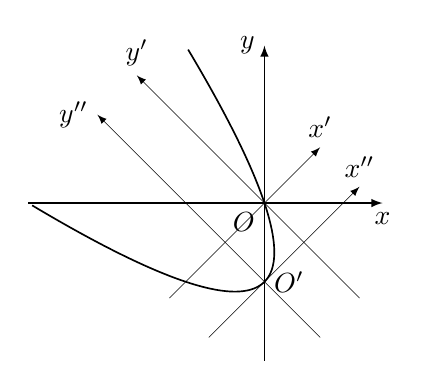
\begin{tikzpicture}[>=latex,scale=1.0,samples=200]
  \draw[thin,->](-3,0)--(1.5,0)node[below]{$x$};
  \draw[thin,->](0,-2)--(0,2)node[left]{$y$};
  \tkzDefPoints{0/0/O,0/-1/O'}
  \tkzLabelPoints[below left](O)
  \tkzLabelPoints[right](O')
  \begin{scope}[rotate=45]
    \draw[very thin,->](-1.707,0)--(1,0)node[above]{$x'$};
    \draw[very thin,->](0,-1.707)--(0,2.293)node[above]{$y'$};
  \end{scope}
  \begin{scope}[yshift=-1cm,rotate=45]
    \draw[very thin,->](-1,0)--(1.707,0)node[above]{$x''$};
    \draw[very thin,->](0,-1)--(0,3)node[left]{$y''$};
    \draw [semithick,domain=-1.4:1.4]  plot (\x,{sqrt(2)*\x*\x});
  \end{scope}
\end{tikzpicture}
\end{document}